\section{Tiny Tapeout 5}
\label{sec:tinytapeout5}

Tiny Tapeout 5 saw another change in the desigh to split the multiplexer into two parts in order to improve performance. As a result of the split the controller was also updated to multiplex between the two halves.
Some other small changes to the multiplexer in Tiny Tapeout 5 included the tweaking, addition, or removal of buffers to improve the STA results.

As each spine segment in Tiny Tapeout 5 is now half as long as in Tiny Tapeout 4, it will exhibit half the capacitance. As a result, upon receipt and testing of fabricated chips we expect to see the round trip latency reduced to around \qty{10}{\ns}.

A bigger change in Tiny Tapeout 5 was the inclusion of of an experimental analog design submission, shown in Fig.~\ref{fig:transmission_gate_TT05}.  This was created to test support for analog and mixed signal designs planned for Tiny Tapeout 6.

\begin{figure}[!t]
\centering
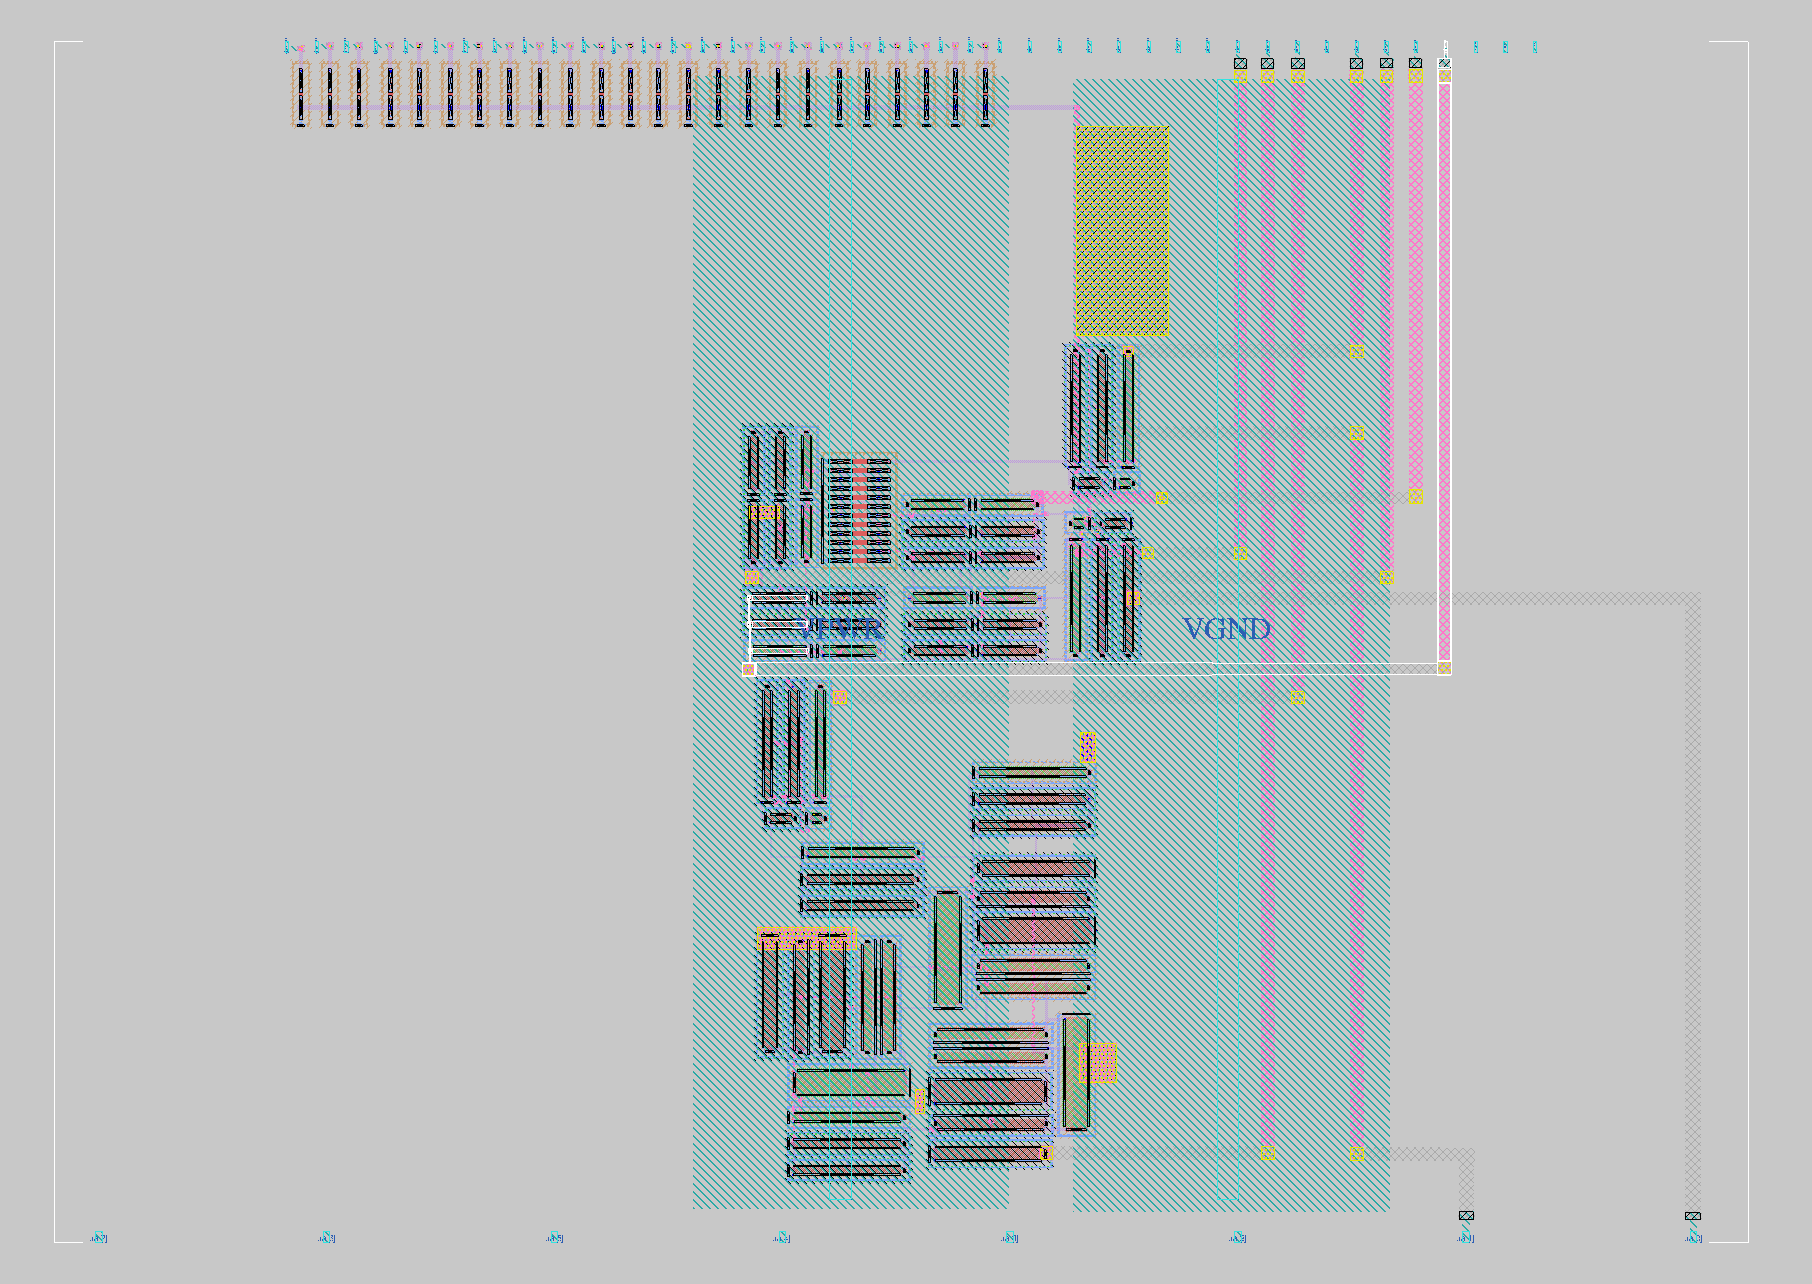
\includegraphics[width=\columnwidth]{./Figs/tt05_transmission_gate.png}
\caption{A ring oscillator and digital to analog converter (DAC) design submitted to Tiny Tapeout 5, with a transmission gate highlighted. This design was automatically placed and routed using an experimental analog place and route (P\&R) tool).}
\label{fig:transmission_gate_TT05}
\end{figure}

%Needs expansion again. Consider merging with TT6?
